\subsection{Filter Stats}\label{HiC:filter-stats} % __02b-filter-stats
%~~~~~~~~~~~~~~~~~~~%
\subsubsection{Input} % inputs
Data from the pipeline \texttt{filter} step is used as input (Section~\ref{HiC:filter}).
%~~~~~~~~~~~~~~~~~~~%
\subsubsection{Analysis} % analysis
Default parameters:
\begin{lstlisting}
params.standard.tcsh$
#!/bin/tcsh

source ./inputs/params/params.tcsh
\end{lstlisting}
%~~~~~~~~~~~~~~~~~~~%
\subsubsection{Output} % outputs
See Figure~\ref{fig:filter-stats-counts} and Figure~\ref{fig:filter-stats-percent}. Default output: %results/filter-stats.standard/filter.by_sample.standard/align.by_sample.bowtie2/all-samples/
\begin{lstlisting}
-rw-r--r-- 1 at570 6.5K Feb 11 15:27 counts.pdf
-rw-r--r-- 1 at570   34 Feb 11 15:27 job.err
-rw-r--r-- 1 at570   47 Feb 11 15:27 job.id
-rw-r--r-- 1 at570   52 Feb 11 15:27 job.out
-rw-r--r-- 1 at570  226 Feb 11 15:27 job.sh
-rw-r--r-- 1 at570 6.7K Feb 11 15:27 percent.pdf
\end{lstlisting}
\begin{figure}[!htb]
    \centering
    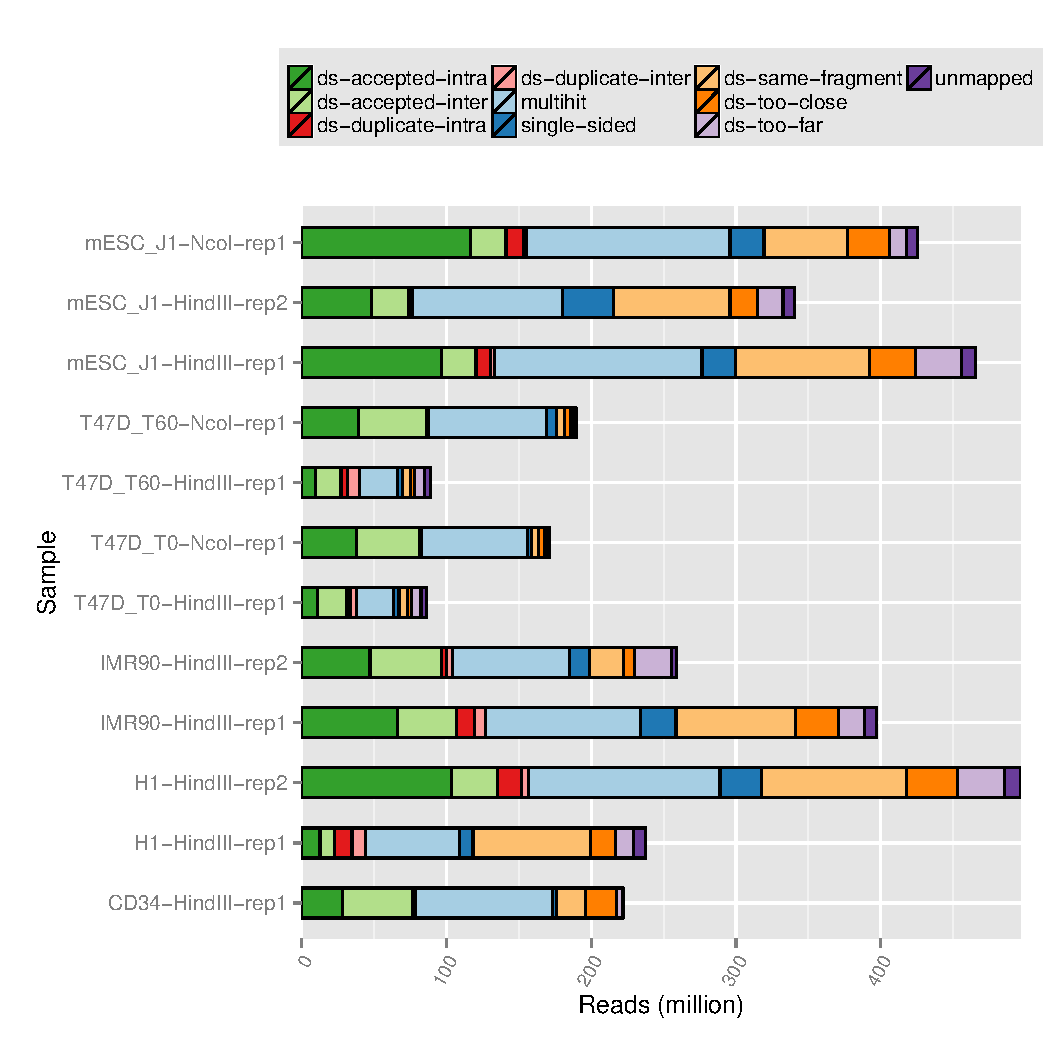
\includegraphics[width=\textwidth,height=\textheight,keepaspectratio]{figure/filter-stats_counts}
    \caption{Filter Stats counts sample output} % results/filter-stats.standard/filter.by_sample.standard/align.by_sample.bowtie2/all-samples/counts.pdf
    \label{fig:filter-stats-counts}
\end{figure}

\begin{figure}[!htb]
    \centering
    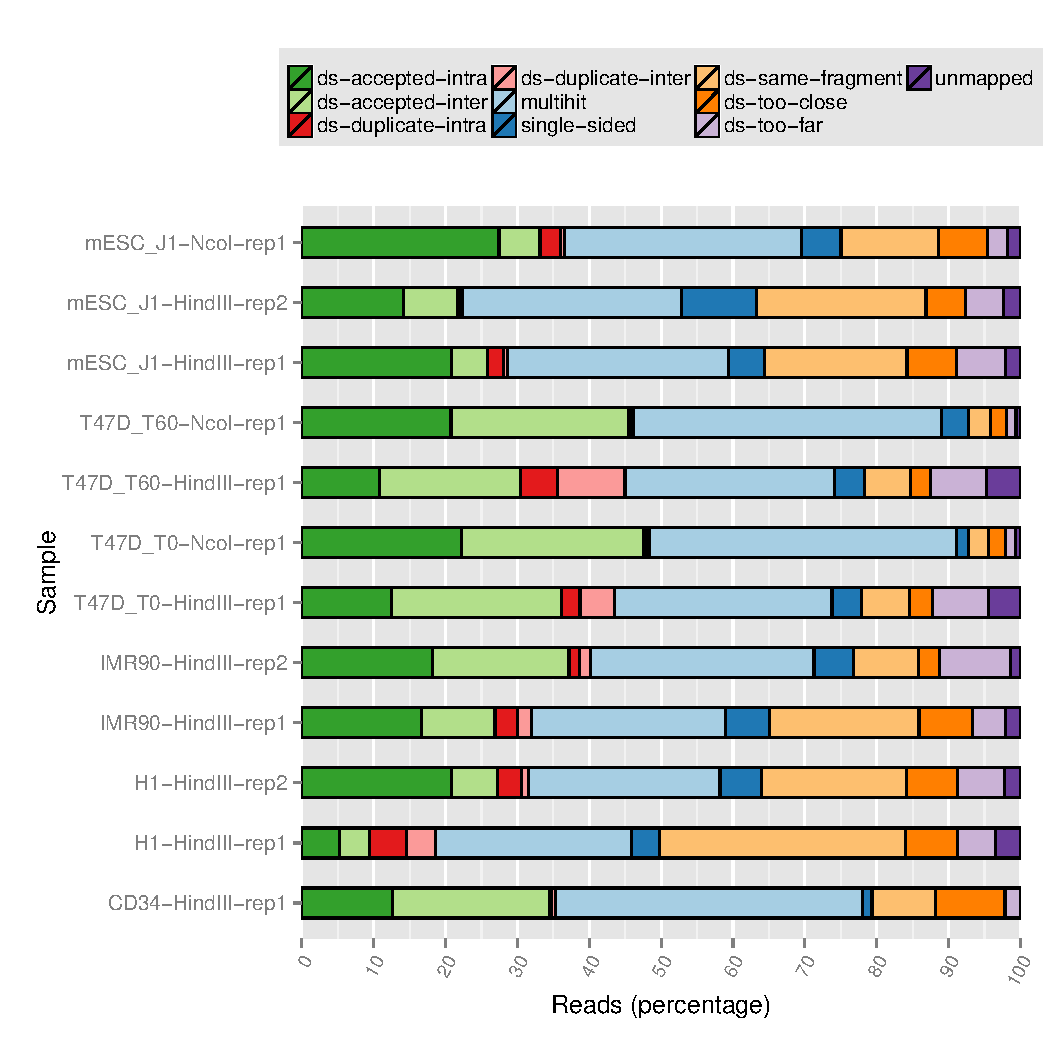
\includegraphics[width=\textwidth,height=\textheight,keepaspectratio]{figure/filter-stats_percent}
    \caption{Filter Stats percentage sample output} % results/filter-stats.standard/filter.by_sample.standard/align.by_sample.bowtie2/all-samples/percent.pdf
    \label{fig:filter-stats-percent}
\end{figure}
% \newpage
\clearpage